%!TEX root = ../elaboration.tex
\chapter{System Proposal}
\label{cha:systemProposal}

\epigraph{
    To achieve the goals set in Chapter \ref{cha:introduction}, this chapter proposes a system architecture that collects and processes the raw data from the \gls{IMU} sensors and transforms it into meaningful metrics, stores it, and then presents it in a clear way to the user.
}

\section{Requirements}
\label{sec:requirements}
With the goals set in Section~\ref{sec:objectives}, and after analyzing the current state of the art, the systems already being used in real life situations and their shortcomings, a set of requirements for the proposed system has to be defined.

It should be able to work indoors, thus avoiding the use of systems like \gls{GPS}, and it should work in any field, without the need of preinstalled structures (like a video system mounted in the court or a set of antennas placed around the court).

It also should provide real-time data of individual game metrics, calculated with the raw data from Wearable Sensors. The purpose of the raw data is to calculate more advanced performance metrics, and should be discarded after being used, so it doesn't waste storage space.

A game of basketball is played by two teams of 5 players, and 8 players at the most can be on the bench, to substitute the ones currently playing.
In order to collect data from all the players of the game, the system should be scalable. The metrics should be calculated and sent to the user, wether collecting data from 1 player, 1 team or 2 teams (with additional substitute players).

Besides storing information about the game metrics, other statistical data should also be stored. Information like box scores, players height, weight and playing position or the teams line-up and coach should be collected for statistical analysis.

The user, whether he is a coach, a player or a fan, should be able to view the processed data and statistics from players, teams and games, in a mobile application. This information should be made available publicly, to be accessed by the developed mobile application, or by any other who wants to consume it.

Initially, the system was being designed to be only one mobile device, which would be in charge of connecting to all the Wearable Sensors, collect and process the data, store it and present it to the end user. Early developments showed that this would require too much processing power for a single device, and that these tasks should be divided in layers: one layer for the data collection and data processing; one layer for data storage and one layer for data presentation. 

Summing up, the main requirements of the system are:
\begin{itemize}
    \item To be able to work indoors
    \item No need for pre-installed infrastructures
    \item Provide real-time game metrics
    \item To be able of scaling, in order to collect data from multiple sensors worn by the players
    \item Store the data collected and processed data, for future statistical analysis
    \item Provide this information to an application, available to coaches to improve their team, or to fans, for fan engagement
\end{itemize}

\section{Architecture}
\label{sec:architecture}
In order to support the collection and processing of raw data in real time, handling the connection to all the devices worn by the players (which could raise up to 30 devices), store all the processed data, handle the frontend application and ensure the communication from the user to the devices, the system should be layered, and built using a 3-tier architecture, with Edge computing.

Edge computing allows that the processing to be near the collection of the data, which takes load off the server, and problems like data transfer and latencies don't interfere. It also enables the parallelization of the computation, distributing the connection to the devices and the processing of the raw data between all the Edge processing units. The layering of the architecture allows that each segment is completely independent in its implementation and operation.

The proposed architecture is shown in Figure~\ref{fig:architectureProposal}, and it is comprised of three segments: \textbf{Edge} - Data Collection and Processing; \textbf{Server} - Data Storage and Application Server; \textbf{Client} - Frontend Application.

The architecture will be explained in more detail in the following subsections.

\begin{figure}
    \centering
    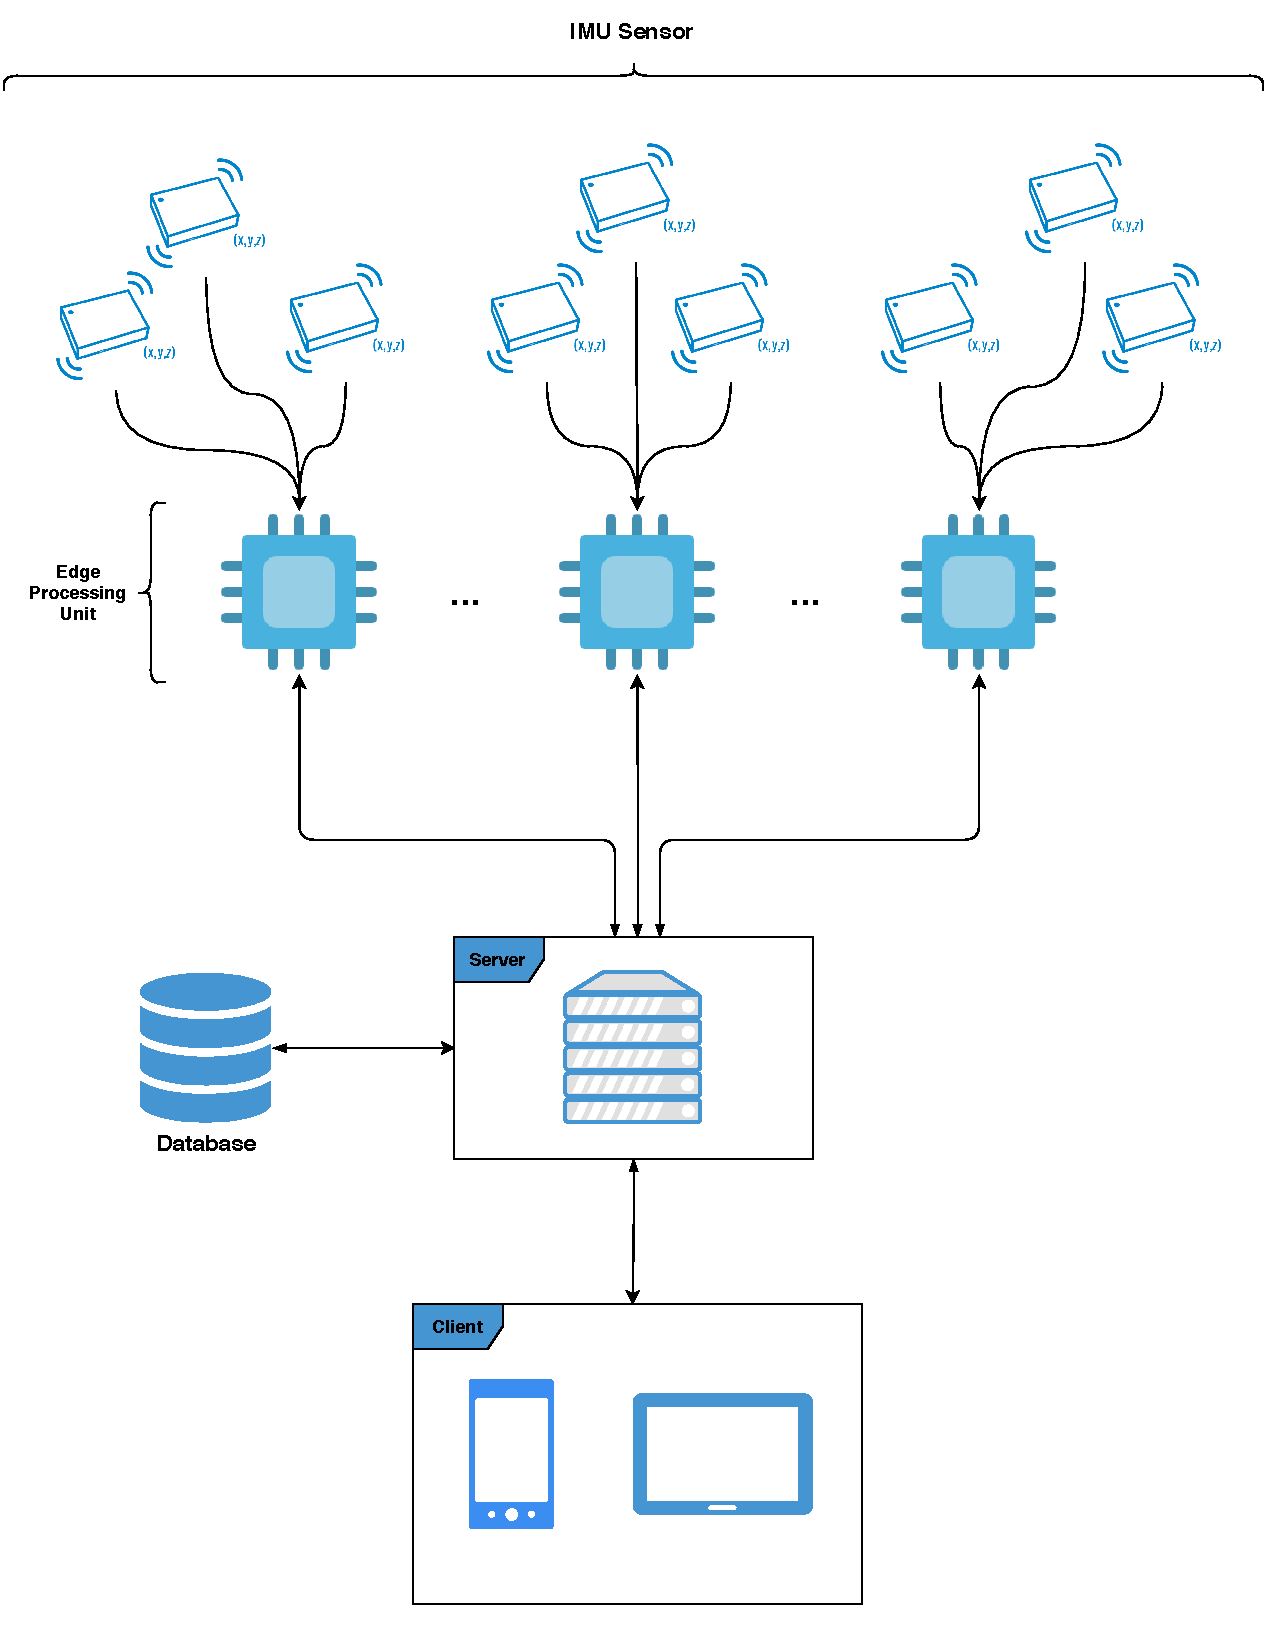
\includegraphics[width=.7\textwidth]{BLESportsTrackerArchitetureProposal.pdf}
    \caption{Proposed Architecture}
    \label{fig:architectureProposal}
\end{figure}

\subsection{Edge}
\label{subsec:edge}
The Edge segment is composed of at least one \gls{IMU} Sensor and one \gls{EPU}, that controls and receives information directly from the \gls{IMU} Sensor. The \gls{EPU} should also be capable of calculating insightful metrics, calculated with the raw data acquired from the \gls{IMU} Sensors.

Due to the variable number of players being tracked, and the number of \gls{IMU} sensors placed in each player, the system should be able to collect data from all the \gls{IMU} sensors. The scalability of the system relies on this segment. In order to accommodate the increase of \gls{IMU} sensors used, more \gls{EPU} may need to be used. These should work seamlessly, collecting data from the sensors, performing calculations and sending the data to the Server.

\subsubsection{IMU Sensors}
\label{subsubsec:imu}
A \gls{IMU} Sensor is an integrated sensor package that measures a body's specific force, angular rate and orientation.

Specific force is a measurement of coordinate acceleration, which can be obtained by removing the gravitational acceleration.
It is measured with accelerometers.
Angular rate is the rate at which a body rotates, measured by gyroscopes.
Orientation is a description of how a body is placed in the place it occupies.
Using magnetometers, a body can be oriented relatively to the Earth's magnetic field~\cite{VectorNav}.

For this application, \gls{IMU} Sensors armed with 3-axis accelerometer and gyroscope should be used.

The \gls{IMU} sensors should be attached to the player's body, in different locations (like the back, the foot or the hand), to track different metrics.


\subsubsection{Edge Processing Unit}
\label{subsubsec:epu}
The \gls{EPU} does the "hard work". Besides handling the connection and controlling the \gls{IMU} Sensors operations, like starting and stopping the raw data collection, this unit has to collect the raw data sent by the \gls{IMU} Sensors several times per second, and perform calculations with the gathered raw data to measure in-game metrics, which are then sent to the server, to be stored and shown to the User.

In order to be able to receive data and calculate in-game metrics from all the \gls{IMU} Sensors, one \gls{EPU} may not be sufficient. An array of \gls{EPU}'s, each one connected to different \gls{IMU} Sensors and sending data in parallel to the Server should be used.

\subsection{Server}
\label{subsec:server}
The Server is the main piece of the architecture, allowing the interaction between the User and the \gls{IMU} Sensors.

The Server can send instructions to the \gls{EPU}, controlling the \gls{IMU} Sensors operations.
When data is received from the \gls{EPU}, the Server stores it in a Database, so that it can be shown to the User, through the Client application.

The server should only store processed data. The raw data should only be used in the Edge to perform calculations. This relieves the need to process raw data in the Server, leaving room for a more complex analysis, over a bigger set of data.

The processed data (\textit{e.g.} game metrics) should be stored in a database, alongside with important statistical information from the players, the teams and the games, such as player's age, height and weight, team's name, location and coach, and game's location and date, to show the fans and to be used in future analysis and statistics.

The Server also hosts the Client Application, which communicates tightly with the Server. For this communication, an \gls{API} should be available, to expose system functions to external applications, such as the Client application, or other applications that may use the data collected and stored in the Server.

\subsection{Client}
\label{subsec:client}
The Client Application provides the end user an interface in which he can control and consult information about players, teams and games. This interface should work seamlessly in multiple platforms, providing a similar user experience no matter the device being used. The preferred method to use the application should be mobile.

This interface should offer different operations and views for different types of users. Fans could consult more generic metrics and statistics, while a coach could manage their team and players, see detailed metrics and statistics of a player, a team or a match, and manage the sensors being used by the players.

The interface should, indirectly, trigger the start and stop of the data collection in the \gls{IMU} Sensors, which will then send the raw data to the \gls{EPU}. After the game metrics are calculated in the Edge, they are shown to the user, in the Client Interface.


%TODO summary